\section{Bluetooth, Classic and Low Energy --- BTC, BLE}

\subsection{Overview}
Bluetooth Classic and Bluetooth Low Energy are similar technologies used for communicating short occasional messages. The former is used, for example, to stream music from a smartphones to wireless headphones; the latter is used with fitness trackers, smart sensors, \dots
It can communicate over quite a long distance ($\thicksim 100m$).
\subsubsection{Physical Layer}
Bluetooth \hl{operates in the $2.4GHz$ band, spanning $80MHz$}. For the modulation, it uses Gaussian Frequency Shift Keying (GSFK) and the bit-rate ranges from $125\,{kbps}$ to $2\,Mbps$.
It uses 40 channels with $2\,MHz$ spacing, with $3$ advertising channels and $37$ data channels.

In order to mitigate potential jamming and interferences, \hl{BLE uses frequency hopping}, where each packet is transmitted over a new channel and whose schedule is negotiated during connection establishment.

\begin{figure}[h]
	\centering
	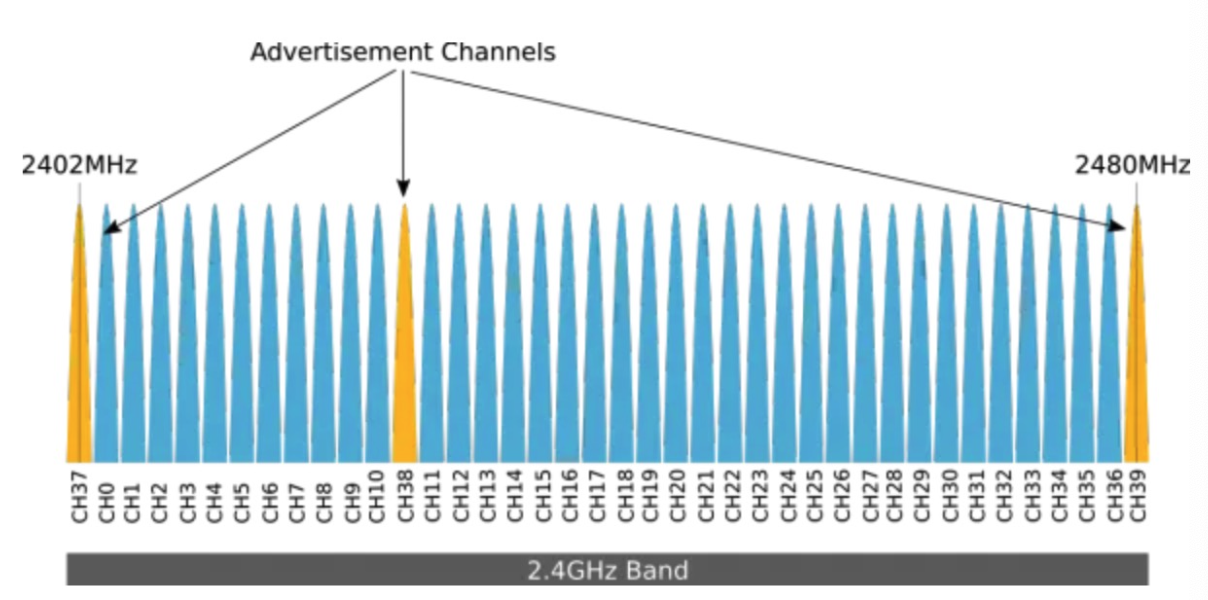
\includegraphics[height=5.3cm]{images/11-ble-comm-band.png}
	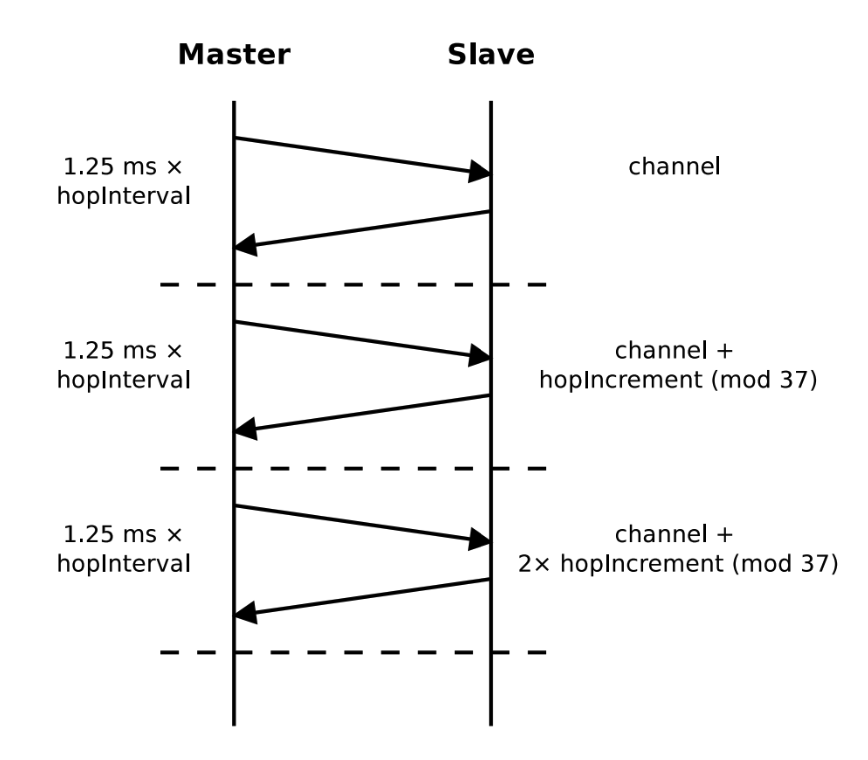
\includegraphics[height=5.3cm]{images/11-fh.png}
	\caption{BLE Communication Band}
	\label{fig:ble-comm-band}
\end{figure}

\subsubsection{Connection Establishment}
The server (a fitness tracker) \hl{periodically broadcasts advertisements}, telling neighboring devices that it's available for pairing. This \hl{advertisement is sent to all $3$ advertisement channels} every $20ms-10s$ and contains a randomized MAC address to identify the device.
When the client (a smartphone) wants to pair with the server, it starts scanning for said beacons and starts the connection establishment process, during which keys are exchanged. Once the devices are paired, then the data flow can begin, regulated by the server's policies for Access Type (R, W, RW) and Security Level (none, Enc, Enc and Auth).

\subsubsection{Pairing}
Besides Legacy Pairing, which is not secure at all, there are 4 Association Methods depending on I/O capabilities: Just Works, Numeric Comparison, Passkey Entry, Out-Of-Band. With a Diffie-Hellman key exchange, the two parties set up a shared Long Term Key (LTK).


\subsubsection{Privacy}
Using a fixed MAC address in every beacon, would make tracking trivial. This is why servers use \hl{address randomization}. There are $3$ different types of random addresses:
\begin{itemize}
	\item static --- may change during bottom
	\item non-resolvable --- may change anytime
	\item \hl{resolvable} --- peers can determine if it belongs to a known device
\end{itemize}

\begin{figure}[h]
	\centering
	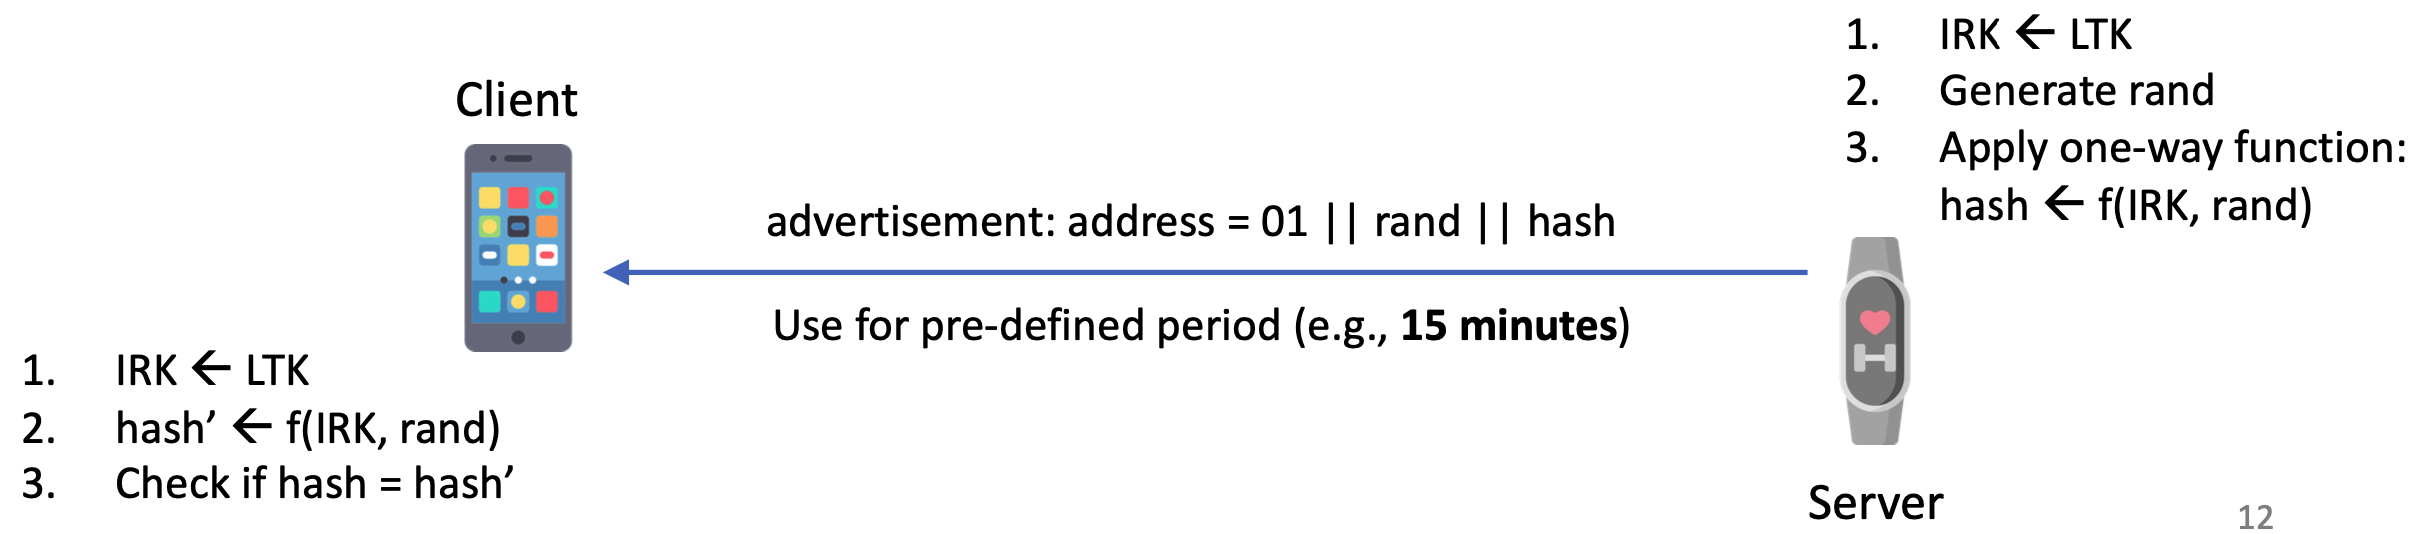
\includegraphics[width=15cm]{images/11-addr-rand.png}
	\caption{BLE Address Randomization}%
	\label{fig:ble-addr-rand}
\end{figure}

\subsection{BLE Security and Privacy}
Attacks to this technology include pairing attacks, data spoofing and user tracking.
\paragraph{Recording communication}
Even though BLE devices use Frequency Hopping, it's been shown that's possible to determine the hopping sequence from on-air traffic by measuring time between two packets on the same channel, the time between two packet on consecutive channels and then solving a few modulo equations. 

\paragraph{Legacy Pairing}
This proprietary protocol can be broken even by passive adversaries who listened to the pairing process of the two devices, since the Secret TK is derived from the PIN, and the PIN is a 6-digit number, the attacker can brute-force it easily.

\paragraph{Secure Connection Pairing}
It uses an authenticated ECDH key exchange. Depending on the device I/O capabilities, only a subset of association methods are available.

\begin{figure}[h]
	\centering
	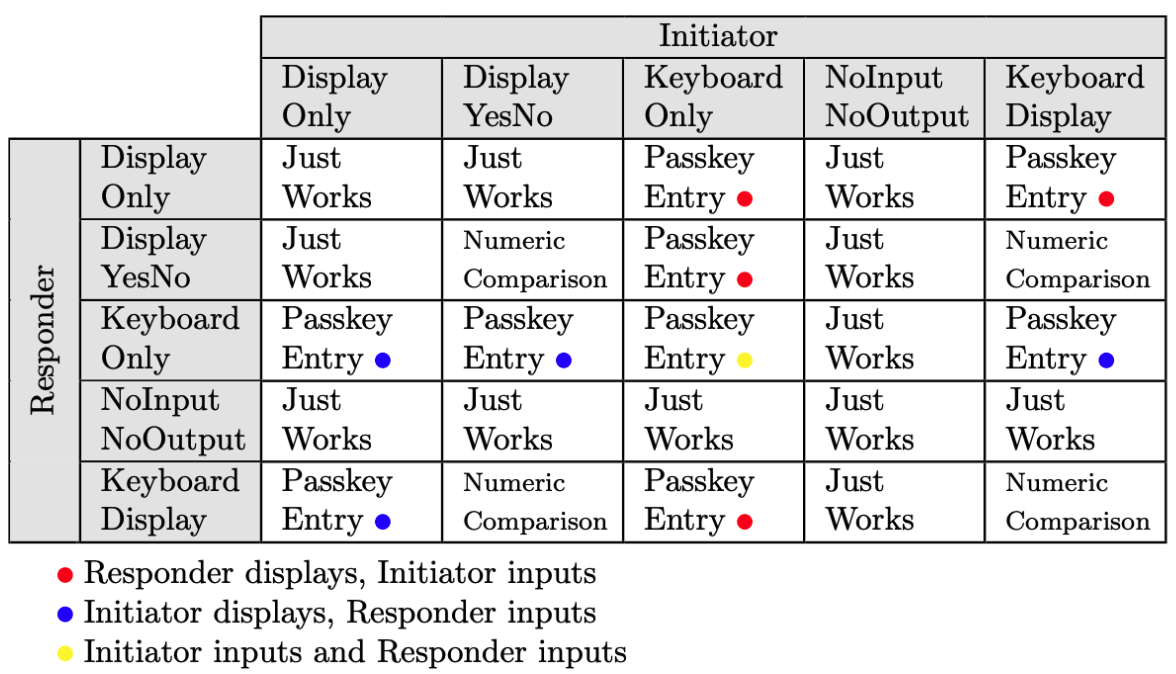
\includegraphics[scale=0.45]{images/11-assoc-methods.png}
	\caption{Association Methods}
	\label{fig:assoc-methons}
\end{figure}

\newpage

The protocol has $4$ phases:
\begin{enumerate}
	\item Feature exchange
	\item Key exchange
	\item Authentication --- depends on the chosen association method
	\item Validation --- checks that everything done in the previous phases went correctly, with no MiTM manipulation
\end{enumerate}

\subsubsection{Method Confusion Attack}
The main idea is that the adversary plays MiTM and uses one association method with the initiator and another one with the responder, then interleaves both protocol runs. this attack works because different association methods use similar "check values". To fix this, it's necessary to make user-copied values incompatible between different methods.

\subsubsection{Data access and spoofing}
If an attribute requires no protection, spoofing/manipulation is possible. Since the authentication can only be required by the server (it's not always on), an adversary, that advertises itself as a benign server, can capture a connection request and the provide spoofed plaintext without, of course, requiring to turn on encryption (as he wouldn't have the key).

\subsubsection{Tracking prevention}
MAC addresses are supposed to change every 15 minutes. However, it's been shown that, for many manufacturers, this only happens once a months.
Also, many devices implement proprietary BLE advertisements to support custom features. If the payload doesn't change as frequently as the MAC randomization, then it's still possible to enable long-term tracking.

\subsection{Digital Contact Tracing}

\paragraph{Goals}
\textit{Complement} manual contact tracing an a pandemic.
Notify users that they have been exposed to a person that tested positive (close than 2m for longer than 15min).
In a timely, scalable, cross-border, yet secure and privacy-preserving manner.
Using existing technologies and existing devices.

\begin{figure}[h]
	\centering
	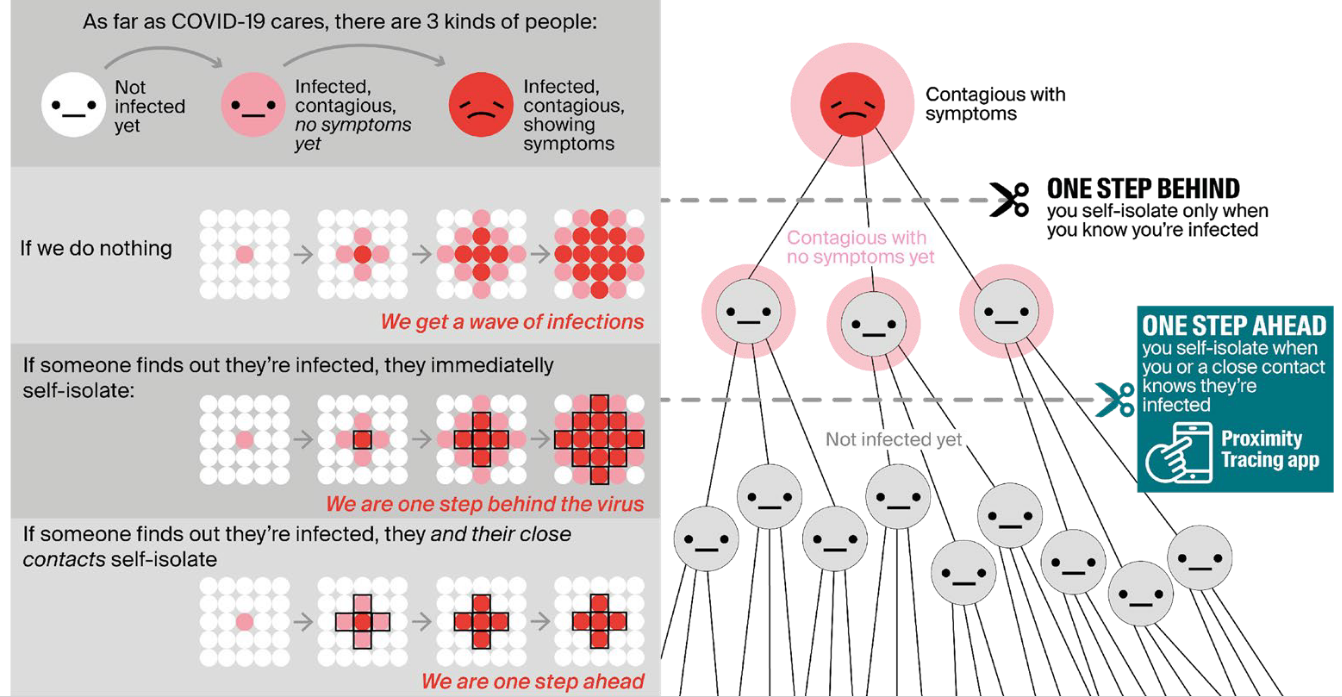
\includegraphics[scale=0.25]{images/11-why-tracing.png}
	\caption{Contact Tracing: Motivation}
	\label{fig:why-tracing}
\end{figure}

\paragraph{Exposure Notification}
Deployed by Apple and Google. Inspired by
\href{https://github.com/DP-3T/documents}{DP-3T}. Used by many countries.

\underline{Idea:}
Phones broadcast ephemeral BLE\footnote{Bluetooth Low Energy} beacons.
Neighbours record beacons.
When infected, phone uploads the beacons to a public board.
Phones poll the public board.

\begin{figure}[h]
	\centering
	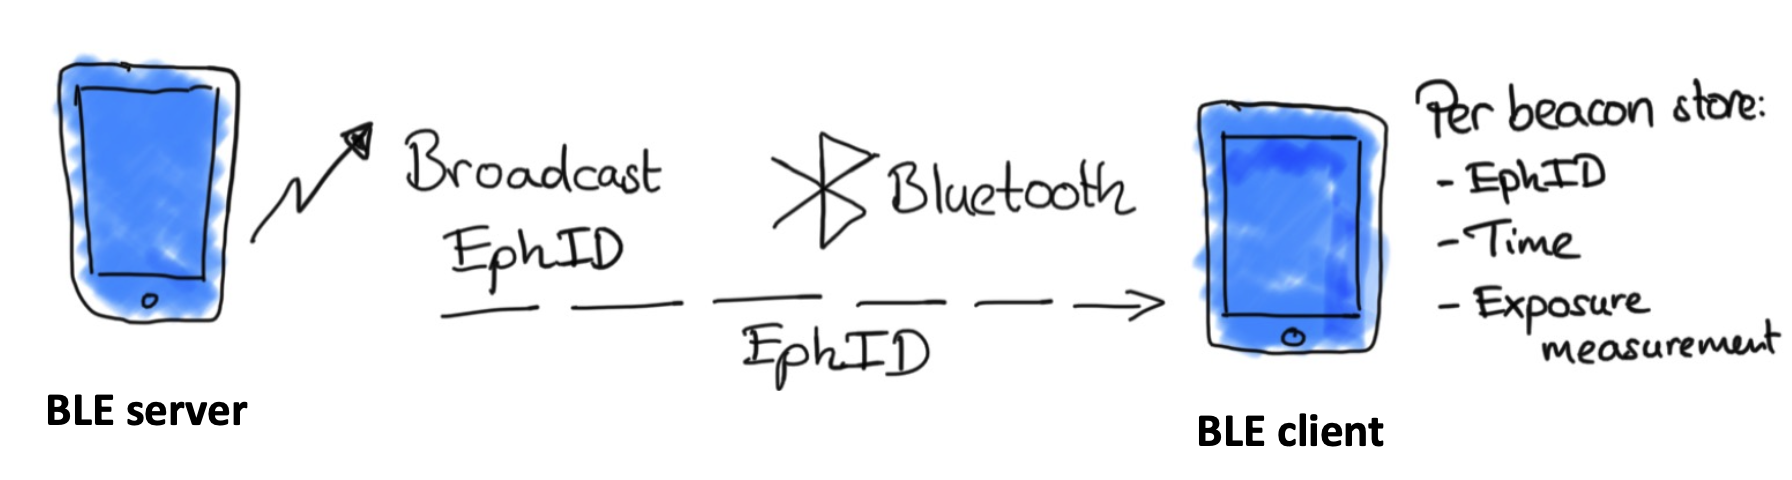
\includegraphics[width=12cm]{images/11-cont-trac-beac.png}
	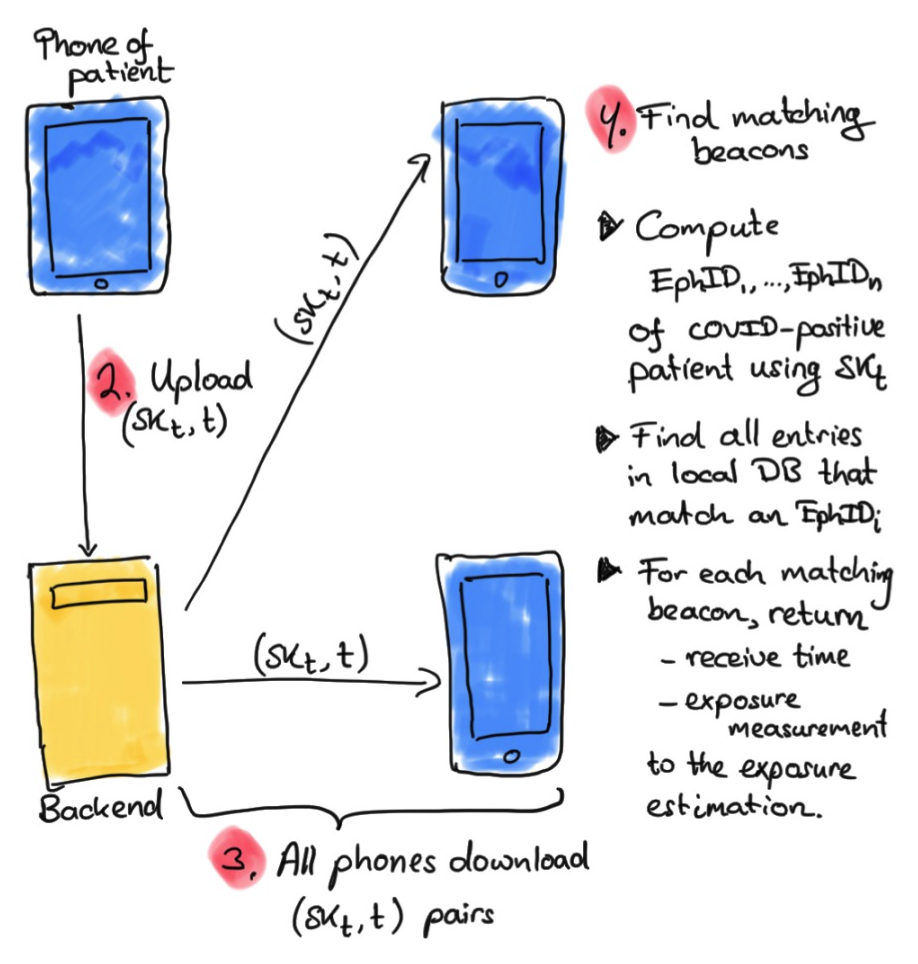
\includegraphics[height=7cm]{images/11-cont-trac-up.png}
	\caption{Contact Tracing: How it works}
	\label{fig:how-tracing}
\end{figure}

\paragraph{DP-3T}
See the
\href{https://github.com/DP-3T/documents/blob/master/DP3T\%20White\%20Paper.pdf}{white
	paper here}.

\paragraph{Open questions}
More evidence is needed in some of the following areas:
\begin{itemize}
	\item How reliable is Bluetooth at estimating proximity?
	\item How reliable are users to respond to a notification or trigger one?
	\item What is the financial impact of self-isolating in response to a notification?
	      What demographics are more likely to comply?
	\item Access to smartphones, digital exclusion of certain groups.
	\item Is digital contact tracing a decisive factor?
	\item Inherent security\footnote{Relay+replay attacks, etc.} and privacy
	      issues\footnote{E.g. if you only met a single person in two weeks and receive a
		      notification, you can reliably de-anonymise them. However, contrast digital
		      (privacy preserving) contact tracing with the data accumulated in manual
		      contact tracing.}
	\item Public communication, building trust.
\end{itemize}